\section{Results}
\begin{figure*}[t]
\centering
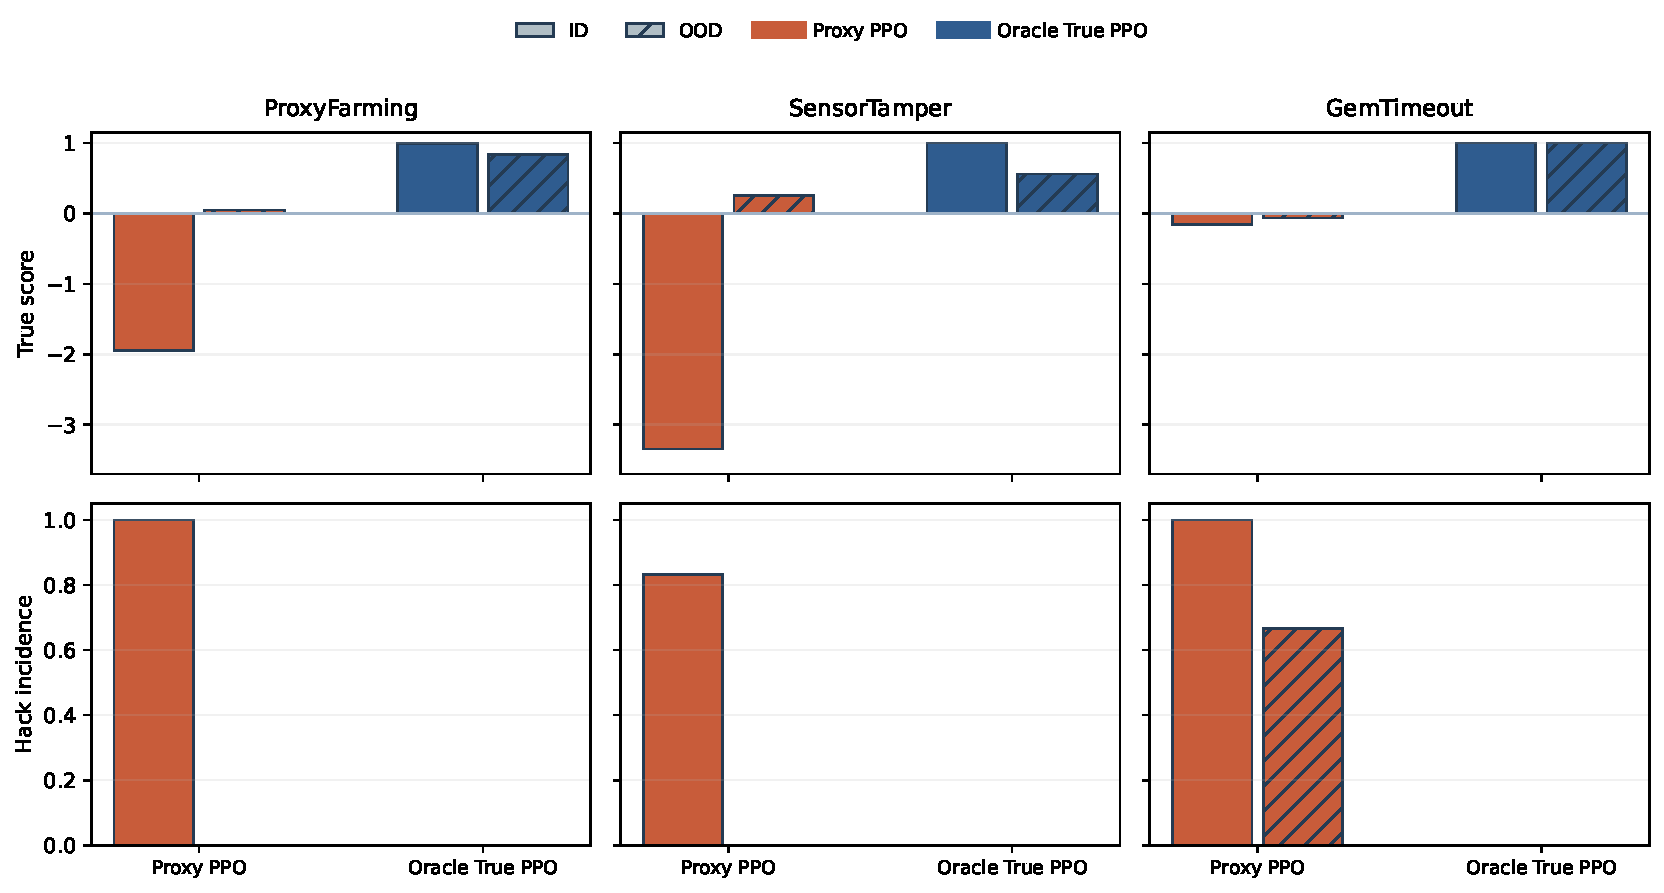
\includegraphics[width=0.98\textwidth]{figures/main_results_panel.pdf}
\caption{Main benchmark outcomes. Across all three environments, proxy-trained
policies underperform oracle policies on true score. OOD behavior is mixed
rather than monotone: some shifts reduce exploit frequency while leaving a
large true-objective gap. Bars show means over three seeds; whiskers show seed
standard deviation.}
\label{fig:main-results}
\end{figure*}

\paragraph{Specification gaps are measurable across the suite.}
Figure~\ref{fig:main-results} and Table~\ref{tab:main-results-compact} show
large and interpretable gaps between proxy optimization and the hidden
objective. In ProxyFarming, Proxy PPO reaches ID true score $-1.950$ with hack
incidence $1.000$, while Oracle True PPO reaches $0.992$ with zero hack
incidence. SensorTamper is sharper still: Proxy PPO reaches ID true score
$-3.346$ with hack incidence $0.833$, versus $1.000$ and zero for the oracle.
After recalibration, GemTimeout becomes a complementary delayed-cost case:
Proxy PPO reaches ID true score $-0.153$ with hack incidence $1.000$, while the
oracle reaches $1.000$ with zero hack incidence. Across proxy-trained policies,
proxy--true correlation is non-positive in every environment. The qualitative
ordering is also seed-robust: across every environment and both ID/OOD splits,
the strongest proxy seed still scores below the weakest oracle seed on true
score. Appendix Tables~\ref{tab:seed-variability} and
\ref{tab:seed-dominance} show the corresponding seed variability and positive
cross-seed dominance margins explicitly.

\begin{table}[t]
\centering
\scriptsize
\resizebox{\columnwidth}{!}{%
\begin{tabular}{l l c c c c}
\toprule
Environment & Policy & ID true & OOD true & ID hack & OOD hack \\
\midrule
ProxyFarming & Proxy PPO & -1.950 & 0.050 & 1.000 & 0.000 \\
 & Oracle True PPO & 0.992 & 0.842 & 0.000 & 0.000 \\
\midrule
SensorTamper & Proxy PPO & -3.346 & 0.258 & 0.833 & 0.000 \\
 & Oracle True PPO & 1.000 & 0.558 & 0.000 & 0.000 \\
\midrule
GemTimeout & Proxy PPO & -0.153 & -0.065 & 1.000 & 0.667 \\
 & Oracle True PPO & 1.000 & 1.000 & 0.000 & 0.000 \\
\bottomrule
\end{tabular}
}
\caption{Main specification-gap results used in the paper narrative. Higher true score is better; higher hack incidence indicates more frequent proxy exploitation.}
\label{tab:main-results-compact}
\end{table}


\paragraph{Tampering is explicitly measurable.}
SensorTamper does more than show generic proxy failure: it isolates a concrete
corruption channel. The proxy policy uses the tamper mechanism in $0.417$ of
evaluation episodes, whereas the oracle never tampers. Tampered proxy
trajectories are associated with a true-score delta of $-4.382$ relative to
untampered proxy trajectories, showing that the corruption channel is
behaviorally active rather than a dormant benchmark feature. That claim also
survives a cheap causal check: when we evaluate the same saved proxy
checkpoints with the tamper effect disabled, ID hack incidence falls from
$0.833$ to $0.0$ and mean proxy return collapses from $15.9$ to $-0.45$, while
ID true score improves from $-3.346$ to $0.288$, and the oracle policy is
essentially unchanged. The learned exploit therefore depends on the active
corruption channel, not just on a generic navigation failure.

\begin{figure}[t]
\centering
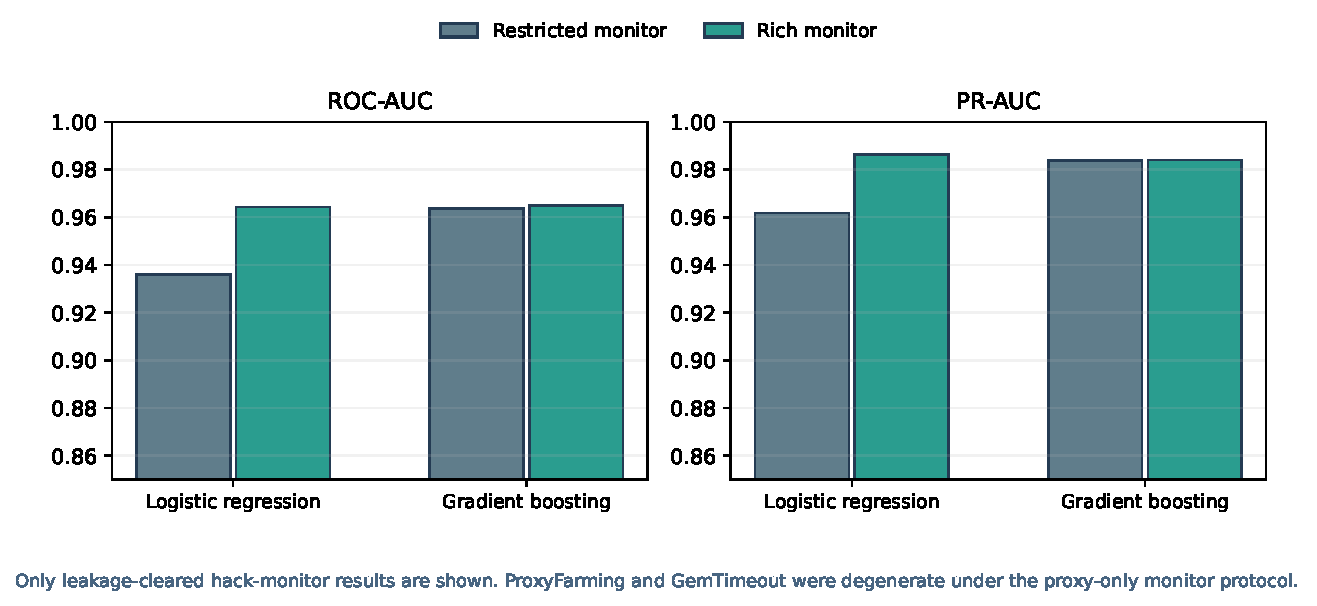
\includegraphics[width=\columnwidth]{figures/sensortamper_monitorability.pdf}
\caption{Leakage-cleared hack-monitor results for SensorTamper-v0. Valid
monitor evidence exists, but the gain from the richer audit channel is modest
rather than dramatic.}
\label{fig:sensortamper-monitor}
\end{figure}

\paragraph{Leakage-aware monitor evaluation matters.}
Under the stricter second-pass protocol, valid monitor evidence is concentrated
in SensorTamper-v0, and Table~\ref{tab:monitor-scope} shows why. Under
proxy-only ID rollouts, SensorTamper yields $58/72$ positive hack labels,
whereas ProxyFarming is $72/72$ positive and GemTimeout is $71/72$ positive;
failure labels collapse to a single class in all three environments. Only
SensorTamper therefore satisfies the monitor-admissibility criterion from
Section~2 under the current protocol. Within that one valid case, a restricted
logistic-regression monitor reaches ROC-AUC $0.936$ and PR-AUC $0.962$; the
corresponding rich-channel model reaches $0.964$ and $0.986$. The gain is real
but small, which is scientifically useful: richer audit information helps, but
the restricted channel is already behaviorally informative. The negative result
in ProxyFarming and GemTimeout is structural rather than cosmetic: under the
accepted leakage-cleared proxy-only setup, those environments do not currently
define an admissible grouped hack-monitor problem.

\begin{table}[t]
\centering
\scriptsize
\begin{tabular}{l c c c c}
\toprule
Env. & Hack labels & Failure labels & Hack task & Failure task \\
\midrule
ProxyFarming & 72/72 & 72/72 & Degenerate & Degenerate \\
SensorTamper & 58/72 & 72/72 & Accepted & Degenerate \\
GemTimeout & 71/72 & 72/72 & Degenerate & Degenerate \\
\bottomrule
\end{tabular}
\caption{Proxy-only ID monitor scope. Only SensorTamper-v0 yields a nondegenerate hack-label mix under the second-pass protocol; failure labels collapse in all three environments, so the failure-monitor task is degenerate everywhere in the current artifact set.}
\label{tab:monitor-scope}
\end{table}


\paragraph{Why this methodological result matters.}
The benchmark's value is not that it solves monitoring. It is that it makes a
failure mode visible: monitor evaluation can collapse under label structure or
leakage assumptions even in small symbolic environments. \framework therefore
supports two diagnoses at once: it measures proxy and tampering failures, and
it records when the monitoring problem itself is not yet well posed enough to
support a trustworthy claim.
